%% The "\appendix" call has already been made in the declaration
%% of the "appendices" environment (see thesis.tex).
%\chapter{Pointless extras}
%\label{app:Pointless}

\chapter{Single Parameter Variations}\label{app:single_parameter_variations}

The $+3\sigma$ variations between the values obtained directly from the universes and those due to the response function in VALOR have been evaluated for all the systematic parameters that are modelled by response functions. The uncorrelated flux variations are shown in \FigureRef{fig:uncorrelated_flux_variations} whereas the proposal and modern interaction parameters are shown in \FigureRef{fig:proposal_variations} and \FigureRef{fig:modern_variations} respectively. All the uncorrelated flux parameters show perfect agreement between the response functions and the universes. Some of the interaction parameters do show some minor differences, however, the differences are small ($<10$ events) which is negligible when compared with the total event rate. 

\def\proposalxsec{
genie_ccresAxial_Genie,genie_ncresAxial_Genie,genie_qema_Genie,genie_NC_Genie,genie_NonResRvpCC1pi_Genie,genie_NonResRvnCC1pi_Genie,genie_NonResRvbarnCC1pi_Genie,genie_NonResRvbarpCC1pi_Genie,genie_NonResRvpCC2pi_Genie,genie_NonResRvnCC2pi_Genie,genie_NonResRvbarnCC2pi_Genie,genie_NonResRvbarpCC2pi_Genie,genie_NonResRvpNC1pi_Genie,genie_NonResRvnNC1pi_Genie,genie_NonResRvbarnNC1pi_Genie,genie_NonResRvbarpNC1pi_Genie,genie_NonResRvpNC2pi_Genie,genie_NonResRvnNC2pi_Genie,genie_NonResRvbarnNC2pi_Genie,genie_NonResRvbarpNC2pi_Genie}

\def\modernxsec {genie_DISAth_Genie,genie_DISBth_Genie,genie_DISCv1u_Genie,genie_DISCv2u_Genie,genie_IntraNukeNabs_Genie,genie_IntraNukeNcex_Genie,genie_IntraNukeNinel_Genie,genie_IntraNukeNmfp_Genie,genie_IntraNukeNpi_Genie,genie_IntraNukePIabs_Genie,genie_IntraNukePIcex_Genie,genie_IntraNukePIinel_Genie,genie_IntraNukePImfp_Genie,genie_IntraNukePIpi_Genie,genie_ResDecayGamma_Genie,genie_ccresVector_Genie,genie_cohMA_Genie,genie_cohR0_Genie,genie_ncelAxial_Genie,genie_ncelEta_Genie,genie_ncresVector_Genie}


\def\uncorrflux  {horncurrent_FluxUnisim,expskin_FluxUnisim,nucleoninexsec_FluxUnisim,nucleontotxsec_FluxUnisim,nucleonqexsec_FluxUnisim,pioninexsec_FluxUnisim, piontotxsec_FluxUnisim,pionqexsec_FluxUnisim}


\begin{figure}
\centering
\foreach \x in \uncorrflux{
\begin{subfigure}[p]{0.185\textwidth}
    \includegraphics[width =\textwidth]{figures-chap6/tweak_nsigma_nue/\x_nuelikeCChigh_3sigma_\x.png}
\end{subfigure}
}
\caption[Flux systematic parameter validation.]{A comparison of the +3$\sigma$ variations from the response functions used by VALOR and the universes for the complete set of uncorrelated flux systematic parameters.}\label{fig:uncorrelated_flux_variations}
\end{figure}

\begin{figure}
\centering
\foreach \x in \proposalxsec{
\begin{subfigure}[p]{0.185\textwidth}
    \includegraphics[width =\textwidth]{figures-chap6/tweak_nsigma_nue/\x_nuelikeCChigh_3sigma_\x.png}
\end{subfigure}
}
\caption[Proposal interaction systematic parameter validation.]{A comparison of the +3$\sigma$ variations from the response functions used by VALOR and the universes for the complete set of proposal interaction systematic parameters.}\label{fig:proposal_variations}
\end{figure}


\begin{figure}
\centering
\foreach \x in \modernxsec{
\begin{subfigure}[p]{0.185\textwidth}
    \includegraphics[width =\textwidth]{figures-chap6/tweak_nsigma_nue/\x_nuelikeCChigh_3sigma_\x.png}
\end{subfigure}
}
\caption[Modern interaction systematic parameter validation.]{A comparison of the +3$\sigma$ variations from the response functions used by VALOR and the universes for the complete set of modern cross-section systematic parameters.}\label{fig:modern_variations}
\end{figure}

\chapter{Detector Volumes}
\label{app:Detector_Volumes}

The (X, Y, Z) coordinates that define the active and fiducial volumes of each module or \gls{tpc} are shown in \TableRef{table:active_and_fiducial_volumes} for \gls{sbnd}, \gls{microboone}, and \gls{icarus}.

\begin{table}[h!]
%\begin{tabular}{lR{15}cc}
\begin{tabular}{lccc}
 & \multicolumn{1}{c}{X [cm]} & \multicolumn{1}{c}{Y [cm]} & \multicolumn{1}{c}{Z [cm]} \\ \cline{2-4} 
 & \multicolumn{3}{c}{Active Volume} \\ \cline{2-4} 
SBND & -199.15 -- \phantom{-}199.15 & -200.00 -- 200.00 & \phantom{-00}0.00 -- \phantom{0}500.00 \\
MicroBooNE & \phantom{00}-1.55 -- \phantom{-}254.80 & -115.53 -- 117.47 & \phantom{-00}0.10 -- 1036.90 \\
ICARUS Module 1 & -364.49 -- \phantom{0}-67.94 & -173.41 -- 143.41 & -909.95 -- \phantom{0}879.95 \\
ICARUS Module 2 & \phantom{-0}67.94 -- \phantom{-}364.49 & -173.41 -- 143.41 & -909.95 -- \phantom{0}879.95 \\ \cline{2-4} 
 & \multicolumn{3}{c}{Fiducial Volume} \\ \cline{2-4} 
SBND TPC 1 & -190.90 -- \phantom{-00}5.60 & -185.00 -- 185.00 & \phantom{-0}15.00 -- 415.00 \\
SBND TPC 2 & \phantom{-0}10.90 -- \phantom{-}190.90 & -185.00 -- 185.00 & \phantom{-0}15.00 -- 415.00 \\
MicroBooNE & \phantom{00}-1.55 -- \phantom{-}229.80 & \phantom{0}-90.53 -- \phantom{0}92.47 & \phantom{-0}30.10 -- 986.90 \\
ICARUS TPC 1 & -339.49 -- -221.04 & -148.41 -- 118.41 & -879.95 -- 829.95 \\
ICARUS TPC 2 & -218.89 -- \phantom{0}-92.94 & -148.41 -- 118.41 & -879.95 -- 829.95 \\
ICARUS TPC 3 & \phantom{-0}92.94 -- \phantom{-}211.39 & -148.41 -- 118.41 & -879.95 -- 829.95 \\
ICARUS TPC 4 & \phantom{-}214.39 -- \phantom{-}339.39 & -148.41 -- 118.41 & -879.95 -- 829.95
\end{tabular}
\caption[The active and fiducial volumes of the \gls{sbn} detectors.]{The dimensions defining the active and fiducial volumes for each \gls{sbn} detector using their respective coordinate systems.} \label{table:active_and_fiducial_volumes}
\end{table}

\chapter{Reconstruction Performance}
\label{app:reconstruction_performance}

The figures in \ChapterRef{chap:Energy_Reco} showing the reconstruction performance were produced whilst running Pandora in cheating mode in order to decouple the reconstruction methods from inefficiencies within the pattern recognition. If Pandora is instead used without cheating mode enabled, the resolution of the reconstruction algorithms is expected to worsen owing to the fact that the number of hits associated with true and reconstructed information is no longer in perfect agreement. 

With cheating mode no longer enabled in Pandora, the true vs reconstructed energy is shown for all three planes using the ESTAR method in \FigureRef{fig:ESTAR_true_vs_reco_no_cheat}. The fractional energy separation from the collection plane is shown in \FigureRef{fig:frac_res_no_cheat} for all three reconstruction methods.

\begin{figure}[h!]
    \centering
    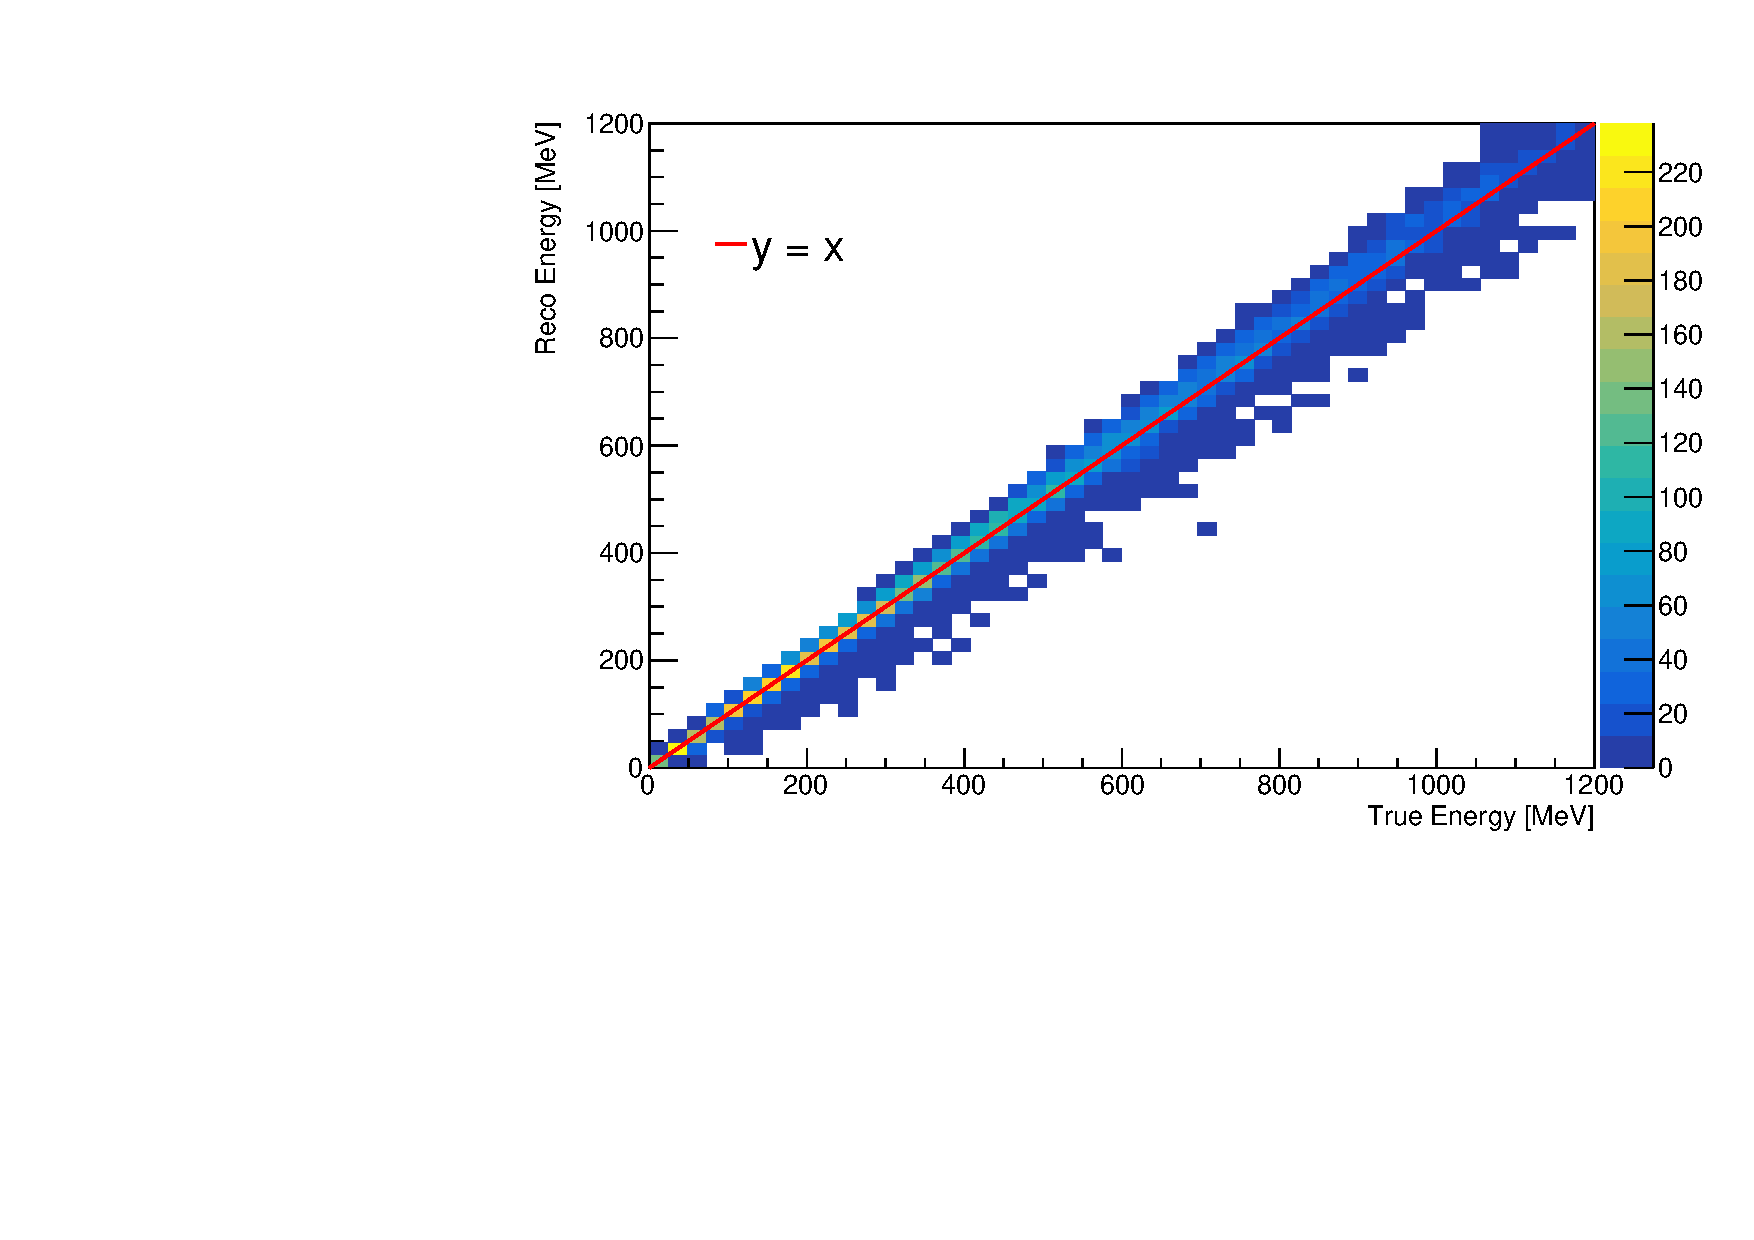
\includegraphics[width = 0.49\textwidth]{figures-chap4/non_cheat/ESTAR_plane0_true_vs_reco.pdf}
    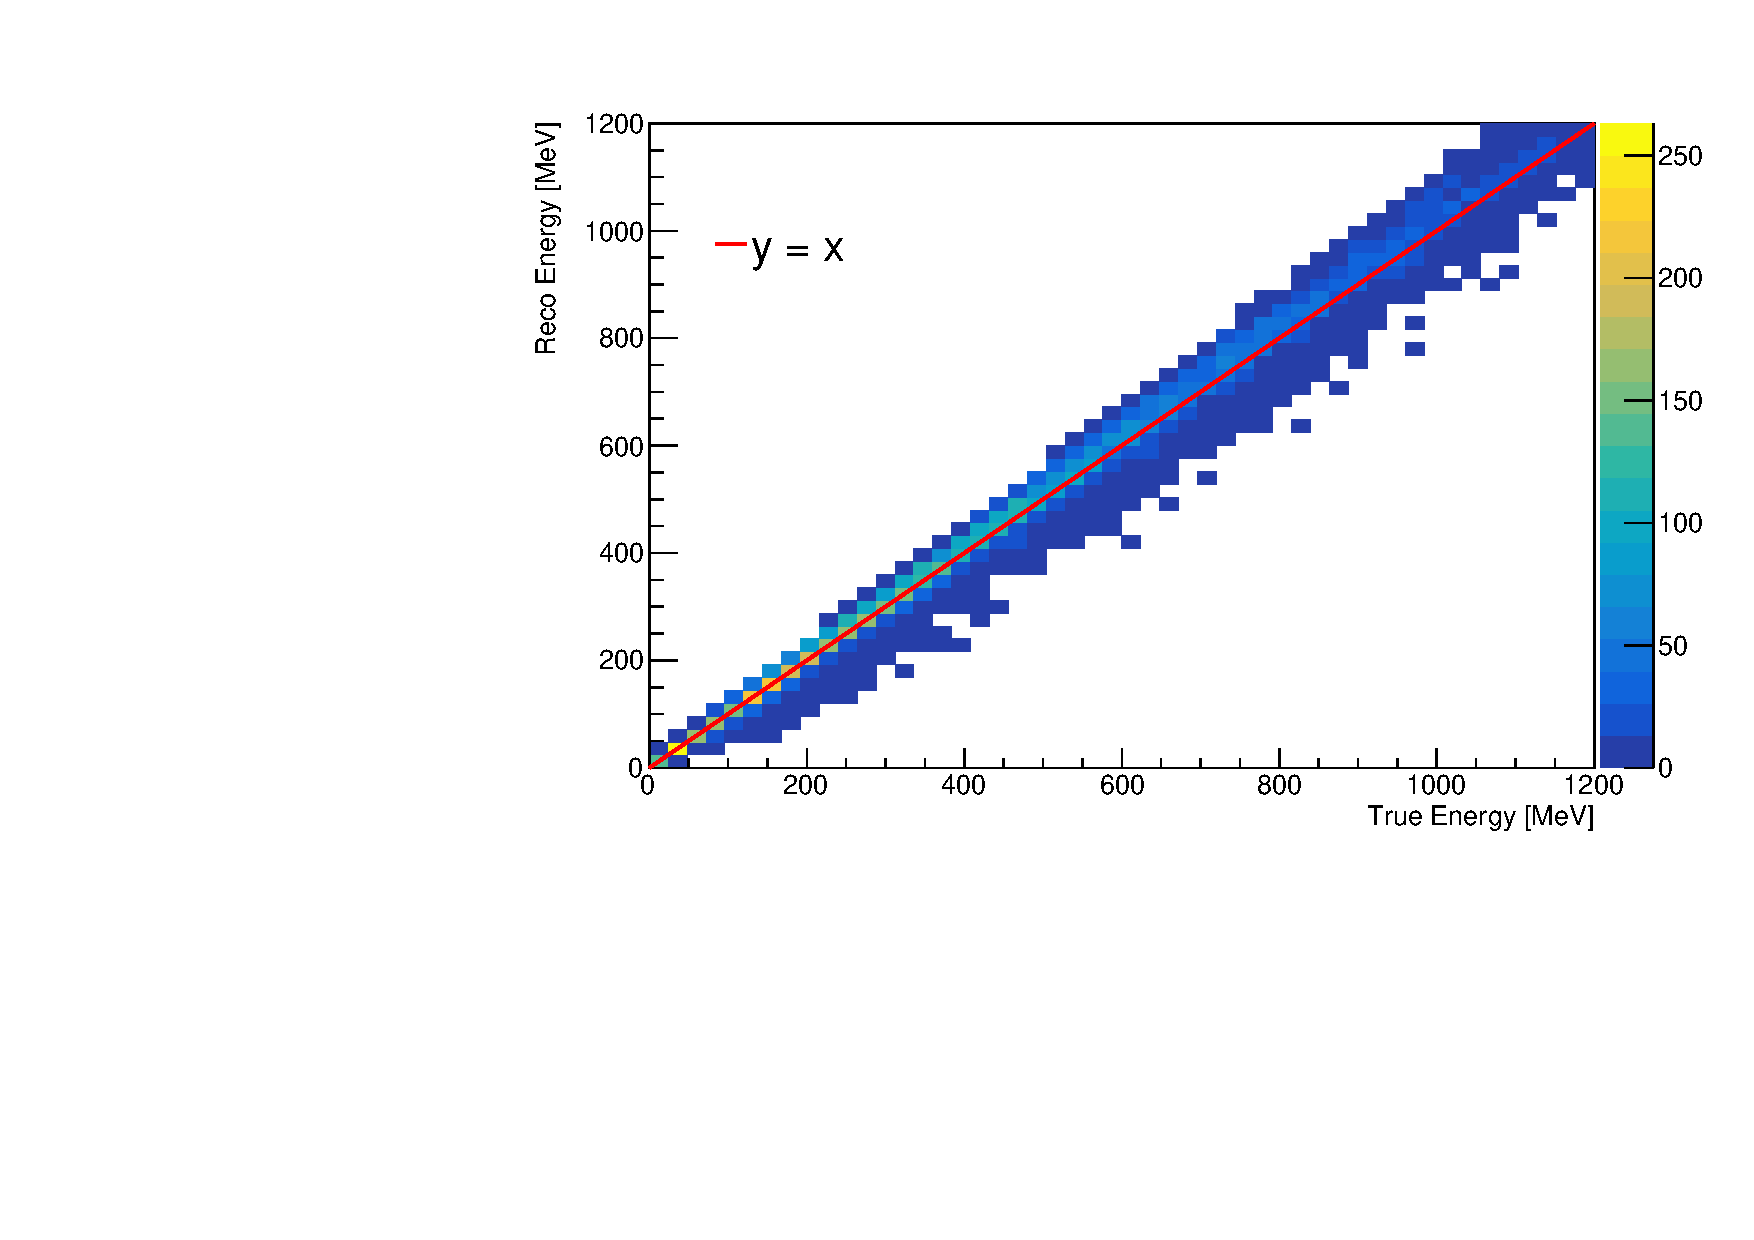
\includegraphics[width = 0.49\textwidth]{figures-chap4/non_cheat/ESTAR_plane1_true_vs_reco.pdf}
    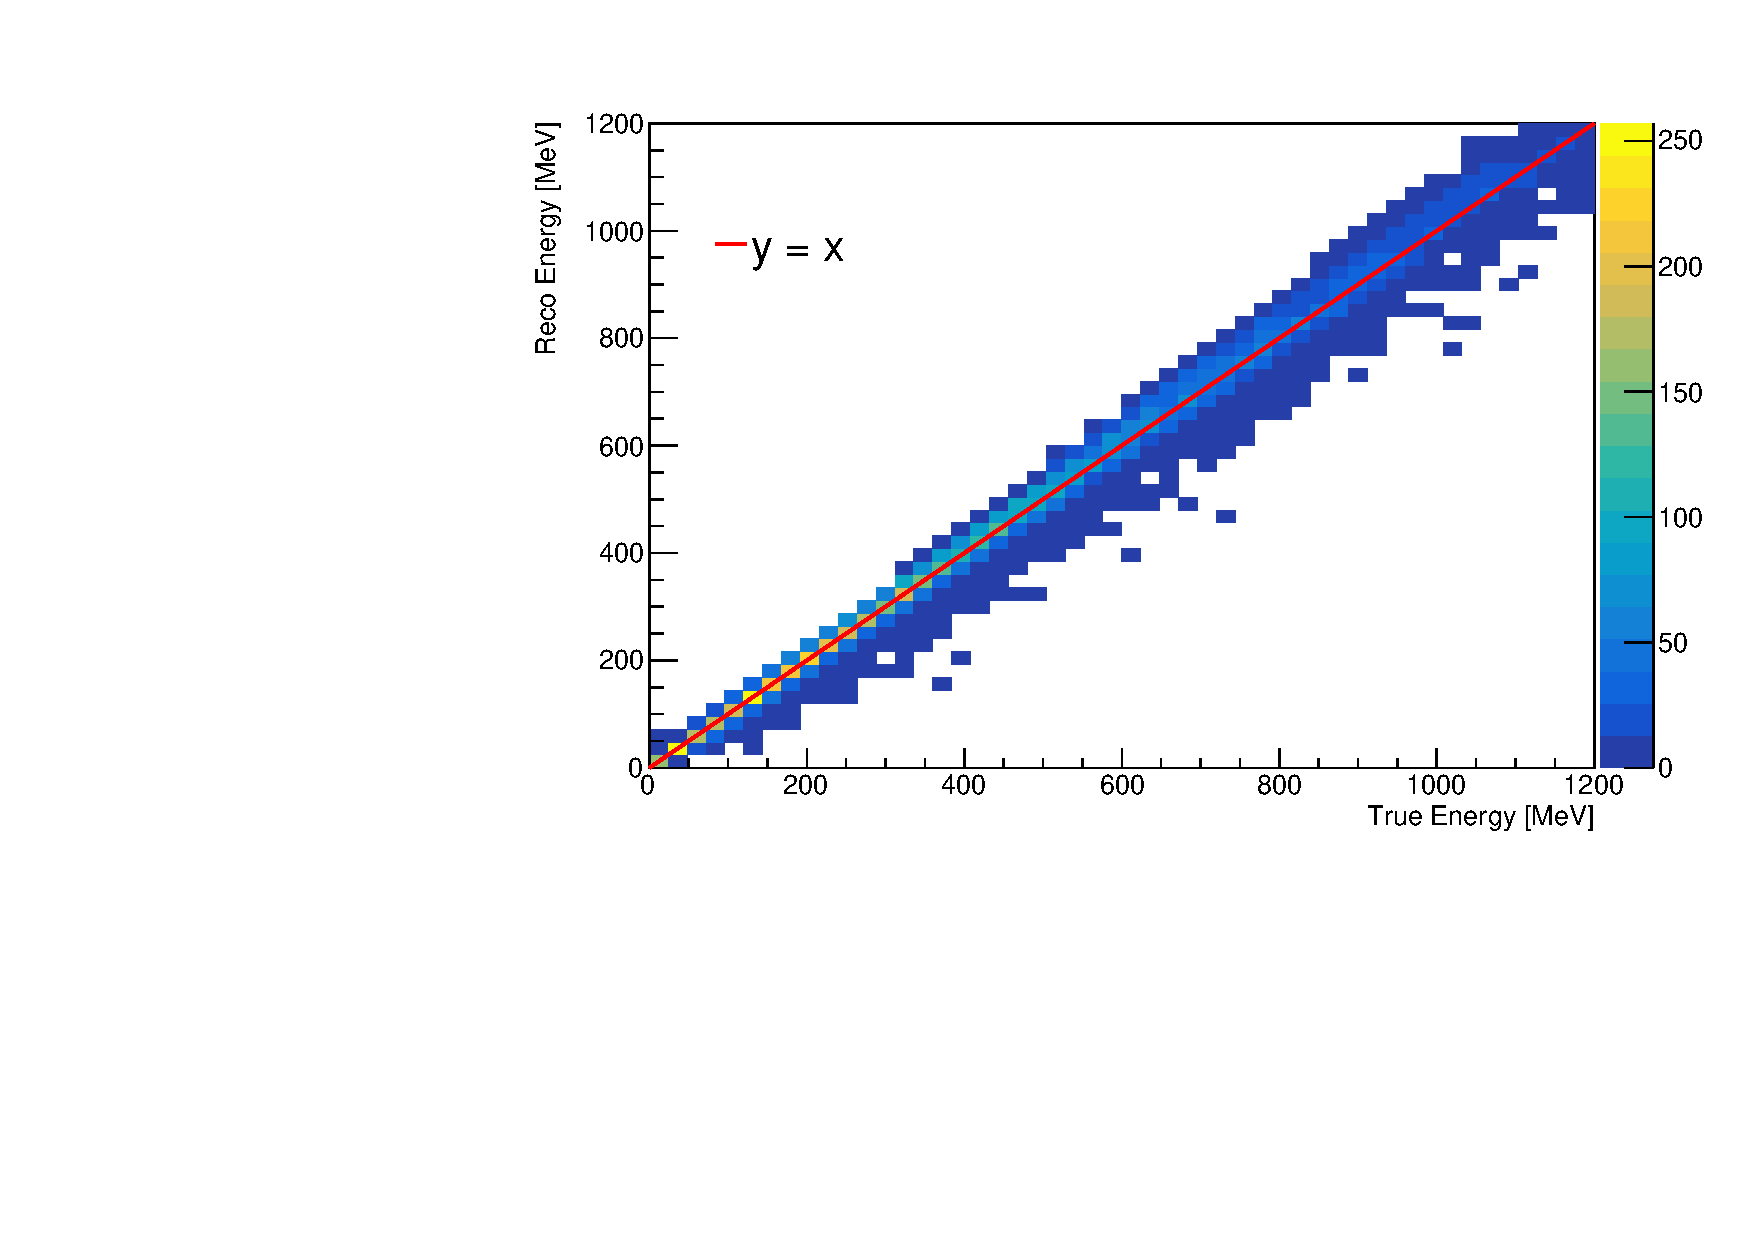
\includegraphics[width = 0.49\textwidth]{figures-chap4/non_cheat/ESTAR_plane2_true_vs_reco.pdf}
    \captionsetup{width=0.45\textwidth}
    \parbox[b]{0.49\textwidth}%
    {
    \caption[True vs reconstructed energy from the ESTAR method without using Pandora in cheating mode.]
    {True vs reconstructed energy from a showering electron. The true energy has been evaluated from the hits of each shower. Pandora was not run in cheating mode. Top Left: Induction plane 0, Top Right: Induction plane 1 and Bottom Left: Collection plane. \\}
    \label{fig:ESTAR_true_vs_reco_no_cheat}}
\end{figure}

\begin{figure}[h!]
    \centering
    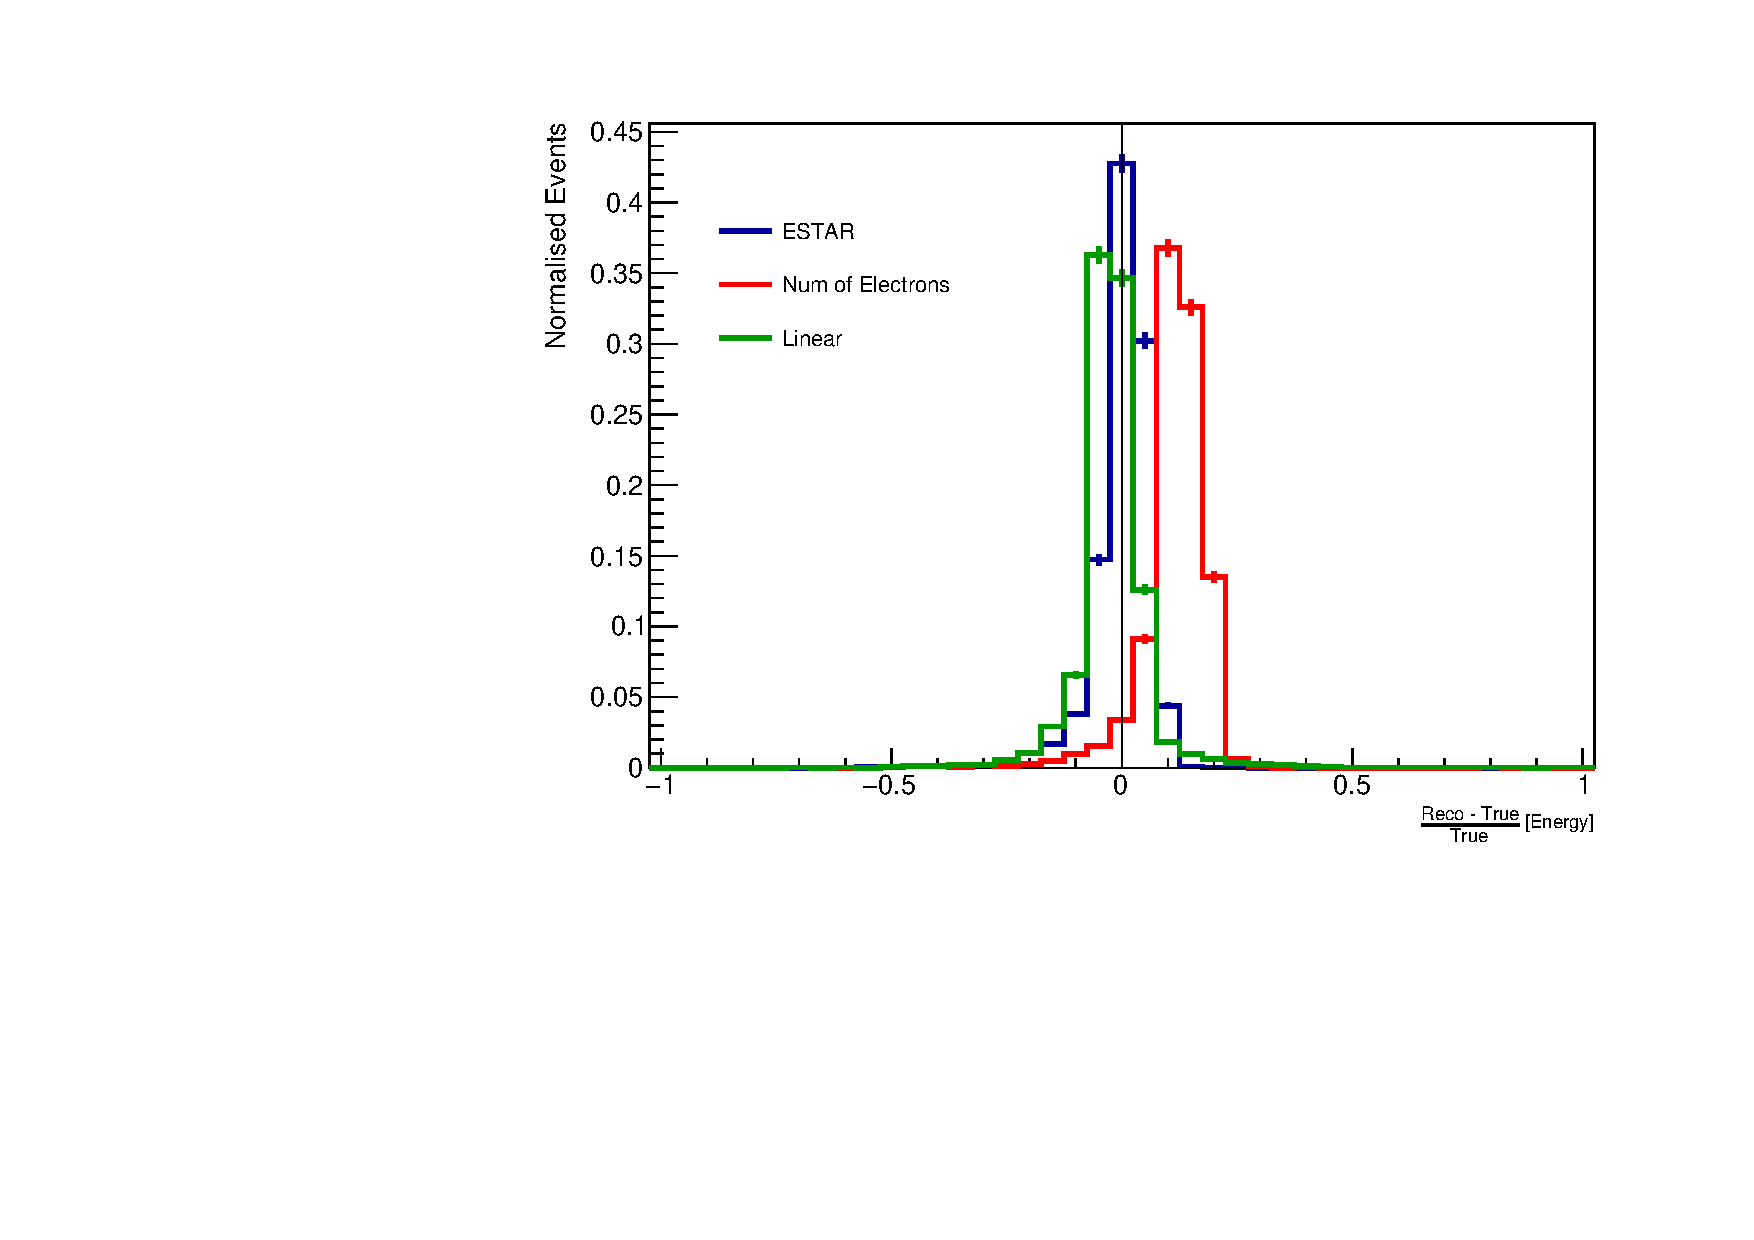
\includegraphics[width = \largefigwidth]{figures-chap4/non_cheat/ESTAR_plane2_frac_res.pdf}
    \caption[Fractional separation of the shower energy with Pandora being run not in cheating mode.]{Comparison of the fractional energy separation from a showering electron for the \textit{Shower Linear Energy tool}, the \textit{Shower Num Electrons Energy tool} and the \textit{Shower ESTAR Energy tool}. The true energy is taken to be the true energy of the available hits and for the reconstruction, Pandora was run whilst not in cheating mode.}
    \label{fig:frac_res_no_cheat}
\end{figure}

Comparing \FigureRef{fig:ESTAR_true_vs_reco_no_cheat} to the ESTAR plot in \FigureRef{fig:reco_vs_true_hit_level} and \FigureRef{fig:true_vs_reco_for_induction_planes}, it can be seen that the energy separation has degraded by disabling cheating mode in Pandora. Similarly, in \FigureRef{fig:frac_res_no_cheat}, each of the distributions has a noticeable tail in the negative x-direction which isn't present in the distributions shown in \FigureRef{fig:fractional_energy_resolution}.


\chapter{\texorpdfstring{\numu Disappearance Analysis}{numu Disappearance Analysis}}\label{app:numu_disapp}

A similar analysis and validation to that described in \ChapterRef{chap:VALOR} that was performed for the two \nue channels was also done for the \numu disappearance channel.

The nominal event rate breakdown for each of the detectors is shown in \FigureRef{fig:numu_disapp_spectra} where an integrated spectrum with oscillation parameters $\sin^2{2\theta_{\mu \mu}} = 0.072$, $\Delta m^2_{41} = 1.32 \text{ eV}^2$ has been overlayed. The overall magnitude of the event rate is several orders of magnitude greater than that for \nue owing to the fact that the \gls{bnb} consists predominantly of \numu. As was the case for \nue disappearance, the reduction in events for \gls{sbnd} is relatively small whereas for \gls{microboone} and \gls{icarus} it is much more significant.

The complete \numu disappearance exclusion sensitivities and allowed regions for both the statistical only case and with the inclusion of flux and interaction systematics are shown in \FigureRef{fig:numu_disapp_global_sensitivity} for the entire \gls{sbn} program alongside external limits from the combined results from \gls{sciboone} and \gls{miniboone}, IceCube, \gls{minos} and its successor \gls{minos}+ \cite{MiniBooNE/SciBooNE_numu_disapp_contour} \cite{IceCube_numu_disapp_contour}\cite{MINOS}\cite{MINOS+}. The results for the \gls{sbn} program are shown at a 5$\sigma$ confidence level whereas the exclusion region from the \gls{sciboone}/\gls{miniboone}, IceCube and \gls{minos}/\gls{minos}+ experiments are shown at the 90\% confidence level. The IceCube experiment also shows an allowed region at the 99\% confidence level. The results from \gls{sbn} show a stronger sensitivity than that obtained by \gls{miniboone}/\gls{sciboone} for all mass splitting values. The exclusion contour is also comparable to that from \gls{minos}/\gls{minos}+ for $\Delta m^2_{41} \gtrsim 1\text{ eV}^2$, however, below this value \gls{minos}/\gls{minos}+ provides a stronger limit. The exclusion contour from IceCube again provides a stronger limit at $\Delta m^2_{41} \lesssim 1\text{ eV}^2$, but for higher values, \gls{sbn} expects to improve on the results from IceCube. The allowed region from IceCube intersects the one from \gls{sbn} so they aren't fully compatible. 

\begin{figure}[h!]
  {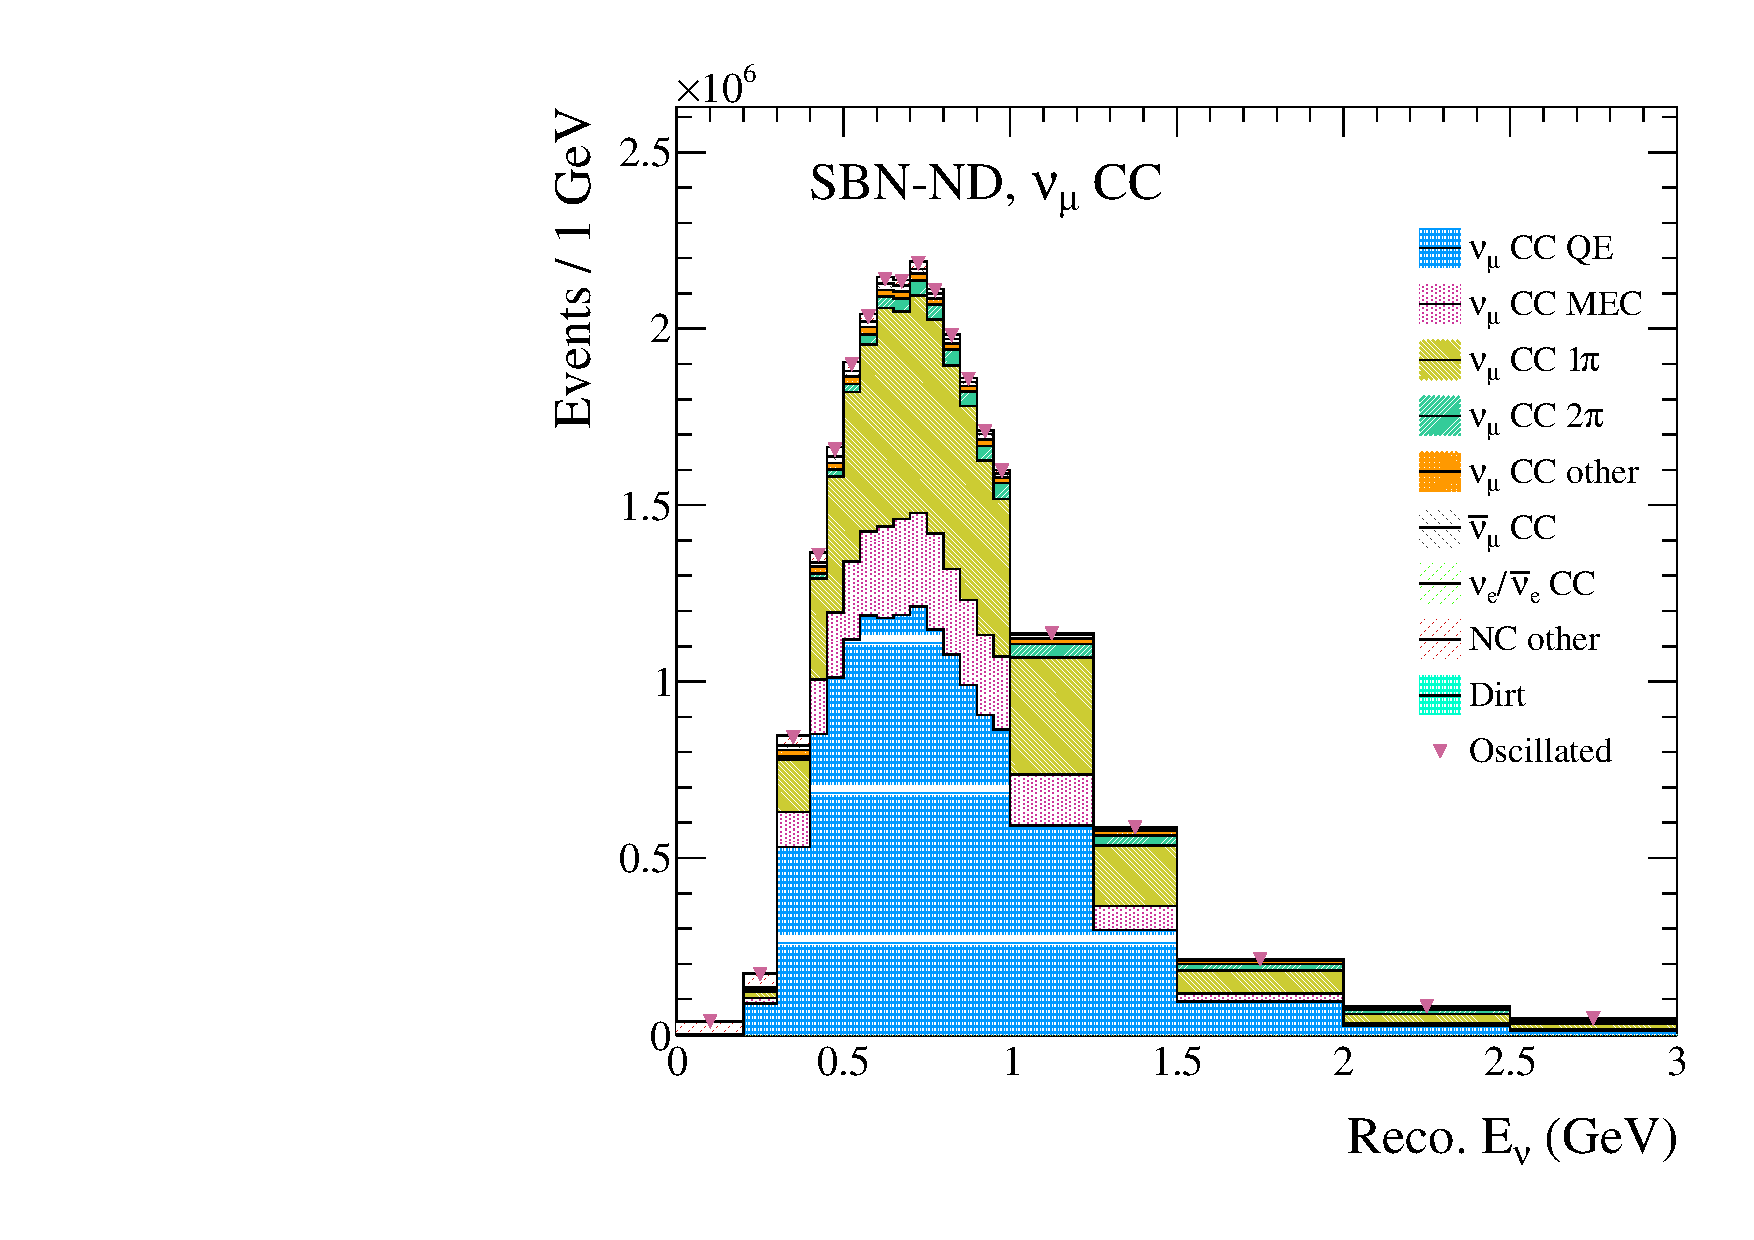
\includegraphics[width=0.49\textwidth]{figures-chap6/spectra/numu_disapp_overlay_dmsq_1.32_sinsq2th_0.072_spectrum_sbn_nd_BNB_FHC_0_modes.pdf}}
  {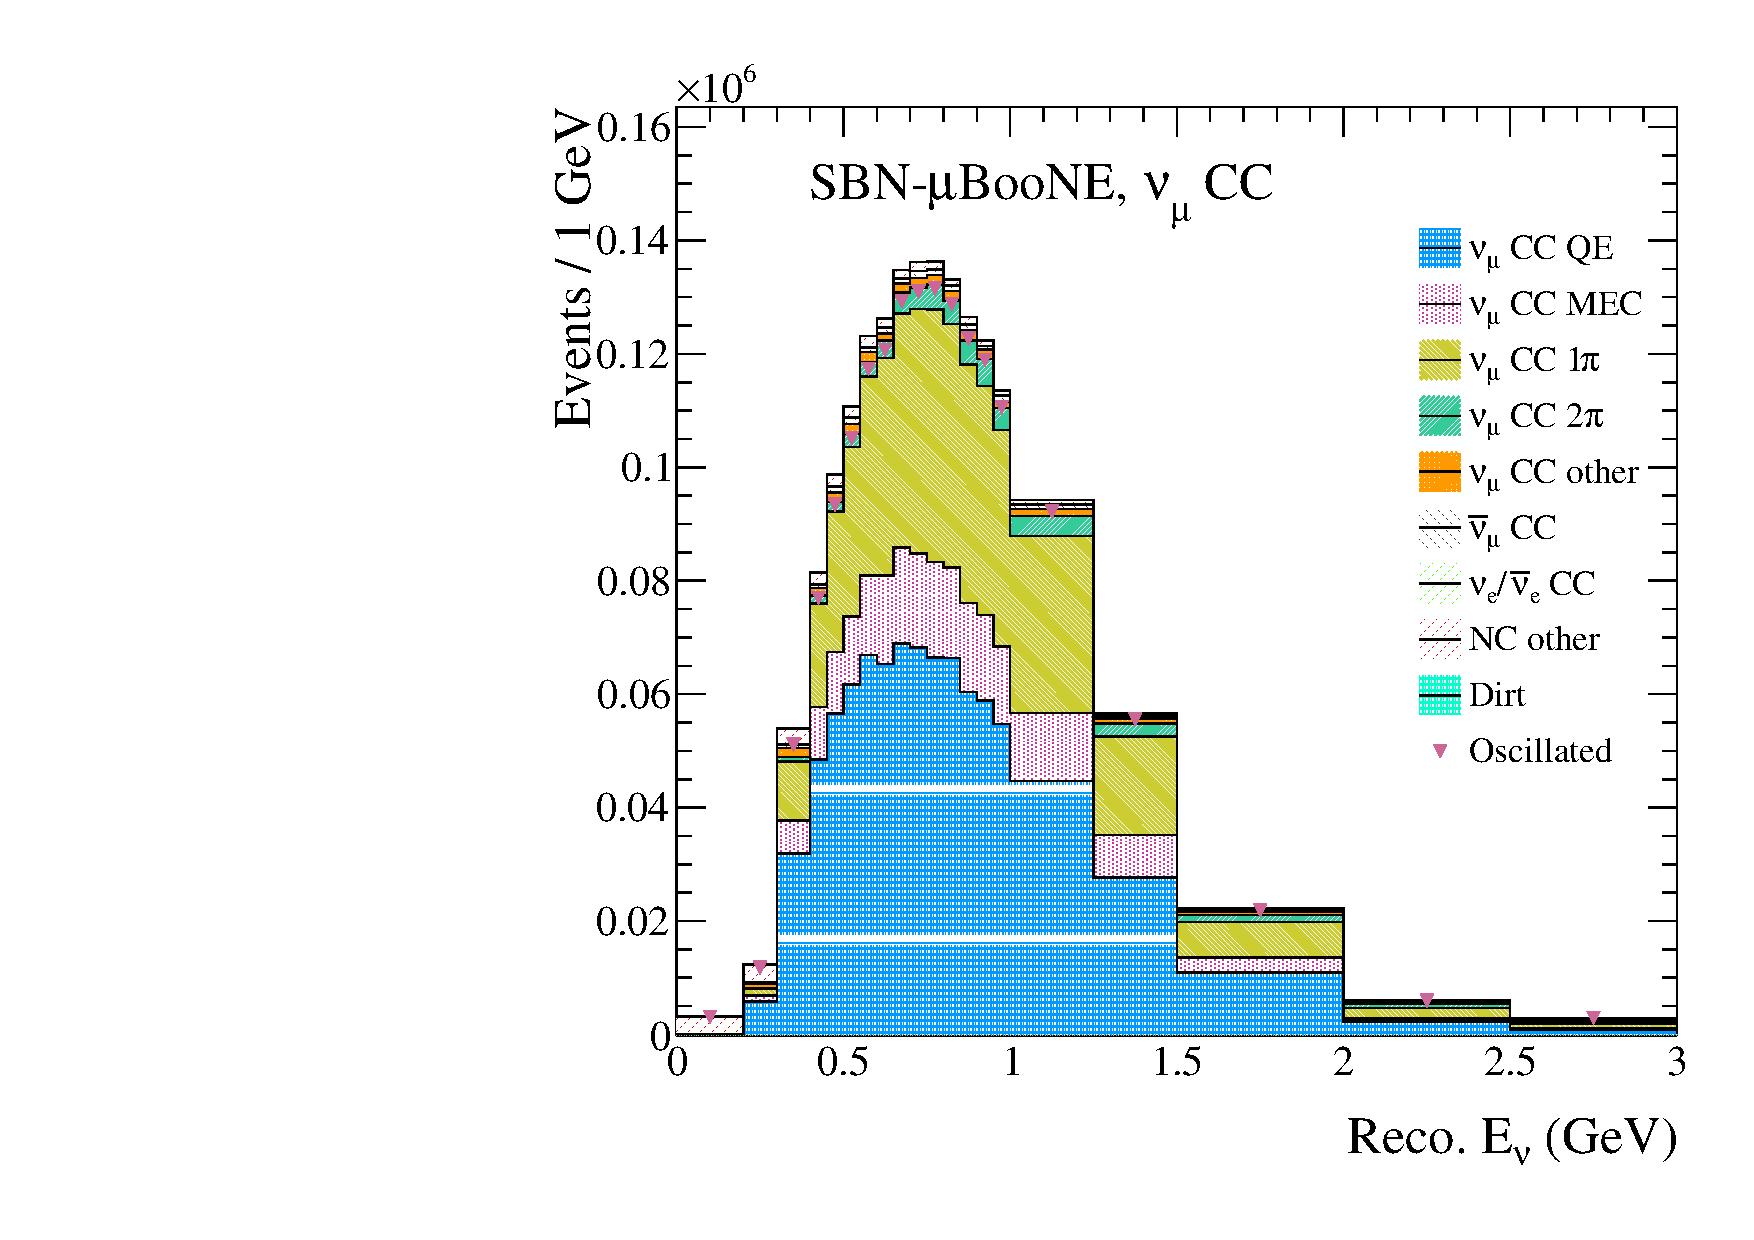
\includegraphics[width=0.49\textwidth]{figures-chap6/spectra/numu_disapp_overlay_dmsq_1.32_sinsq2th_0.072_spectrum_sbn_uboone_BNB_FHC_1_modes.pdf}}
  {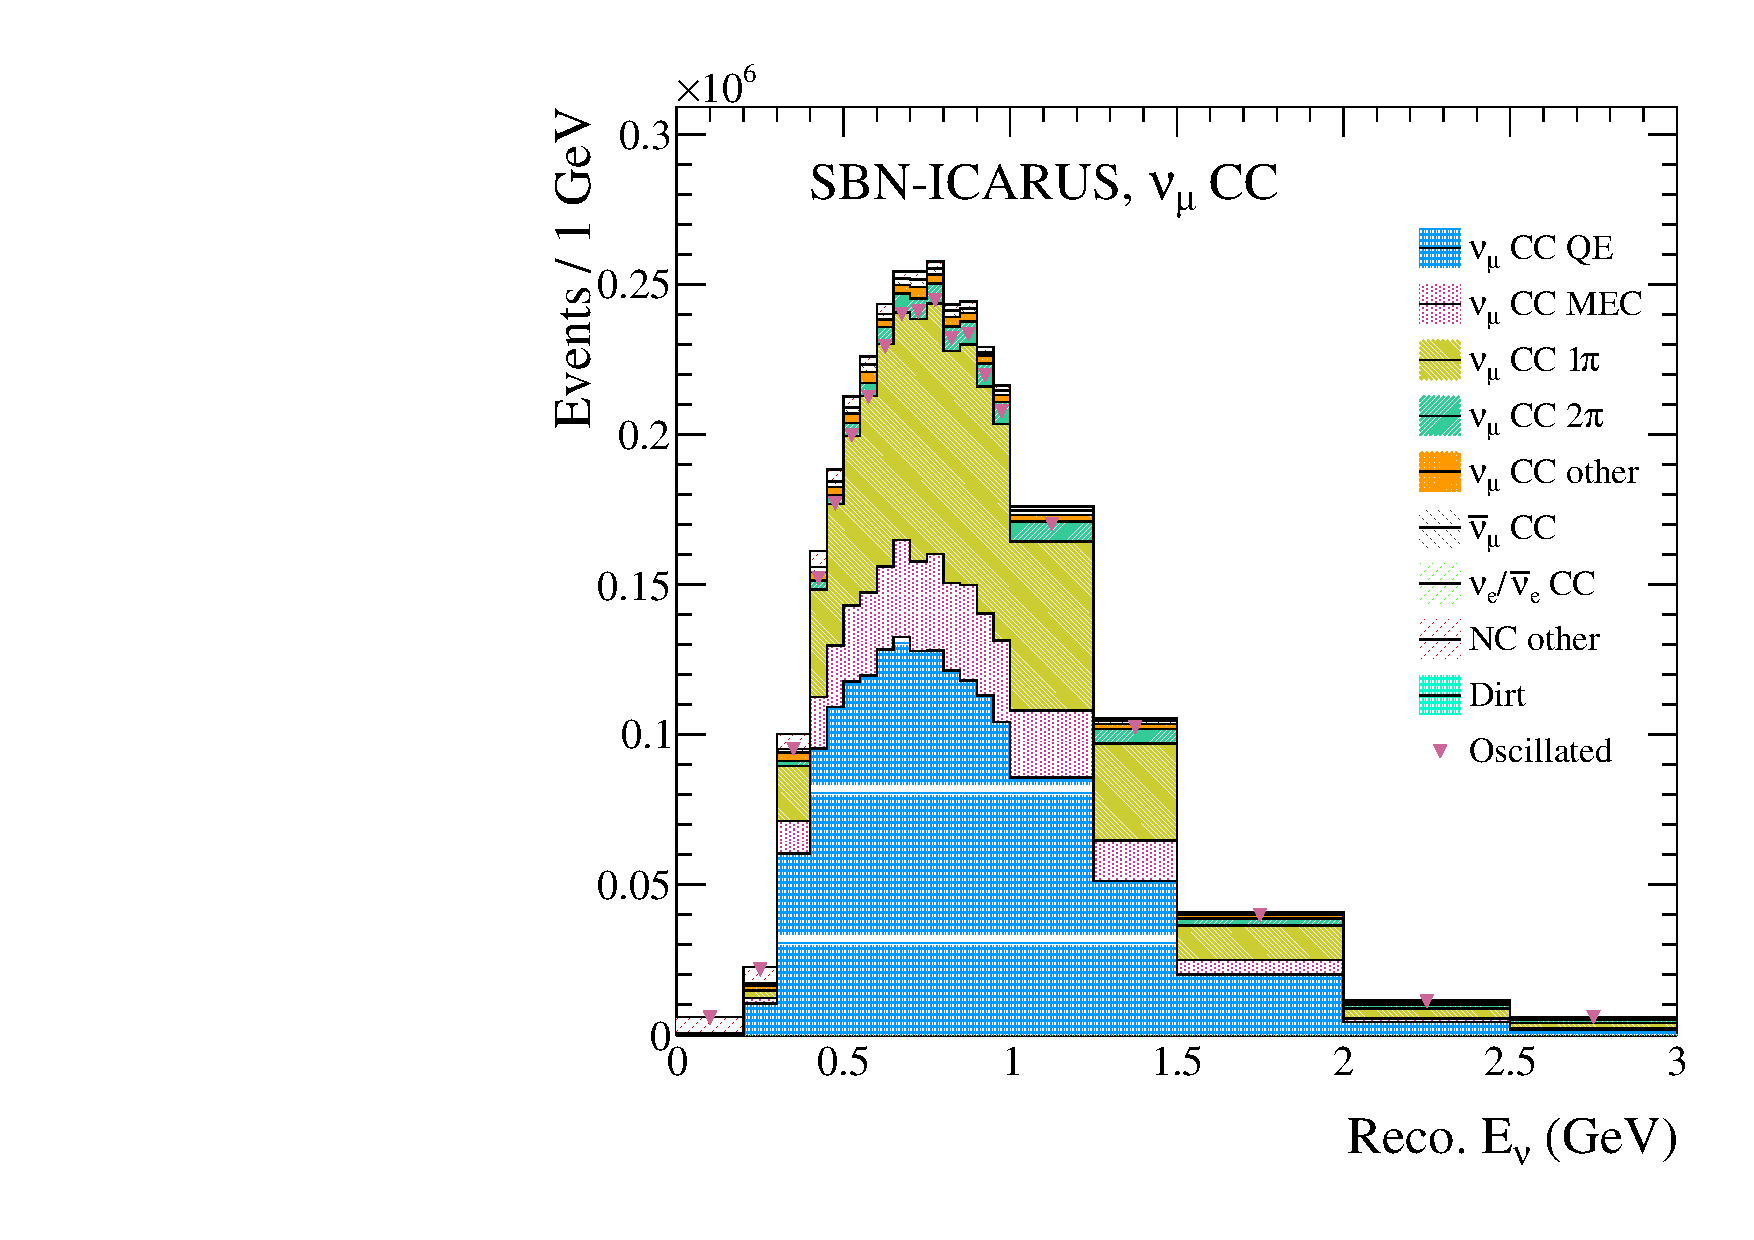
\includegraphics[width=0.49\textwidth]{figures-chap6/spectra/numu_disapp_overlay_dmsq_1.32_sinsq2th_0.072_spectrum_sbn_icarus_BNB_FHC_2_modes.pdf}}
  \captionsetup{width=0.49\textwidth}
  \parbox[b]{0.49\textwidth}%
  {
    \caption[SBN \numu CC inclusive reconstructed neutrino energy spectra with oscillated spectrum overlayed.]{The breakdown of the nominal \numu disappearance spectra overlayed with an integrated oscillated spectrum with oscillation parameters, $\sin^2{2\theta_{\mu \mu}} = 0.072$ and $\Delta m^2_{41} = 1.32$~eV$^2$ showing the decrease in event rate.\\\phantom{.}\\\phantom{.}\\\phantom{.}\\}
    \label{fig:numu_disapp_spectra} 
  }
\end{figure}

\begin{figure}[h!]
    \centering
    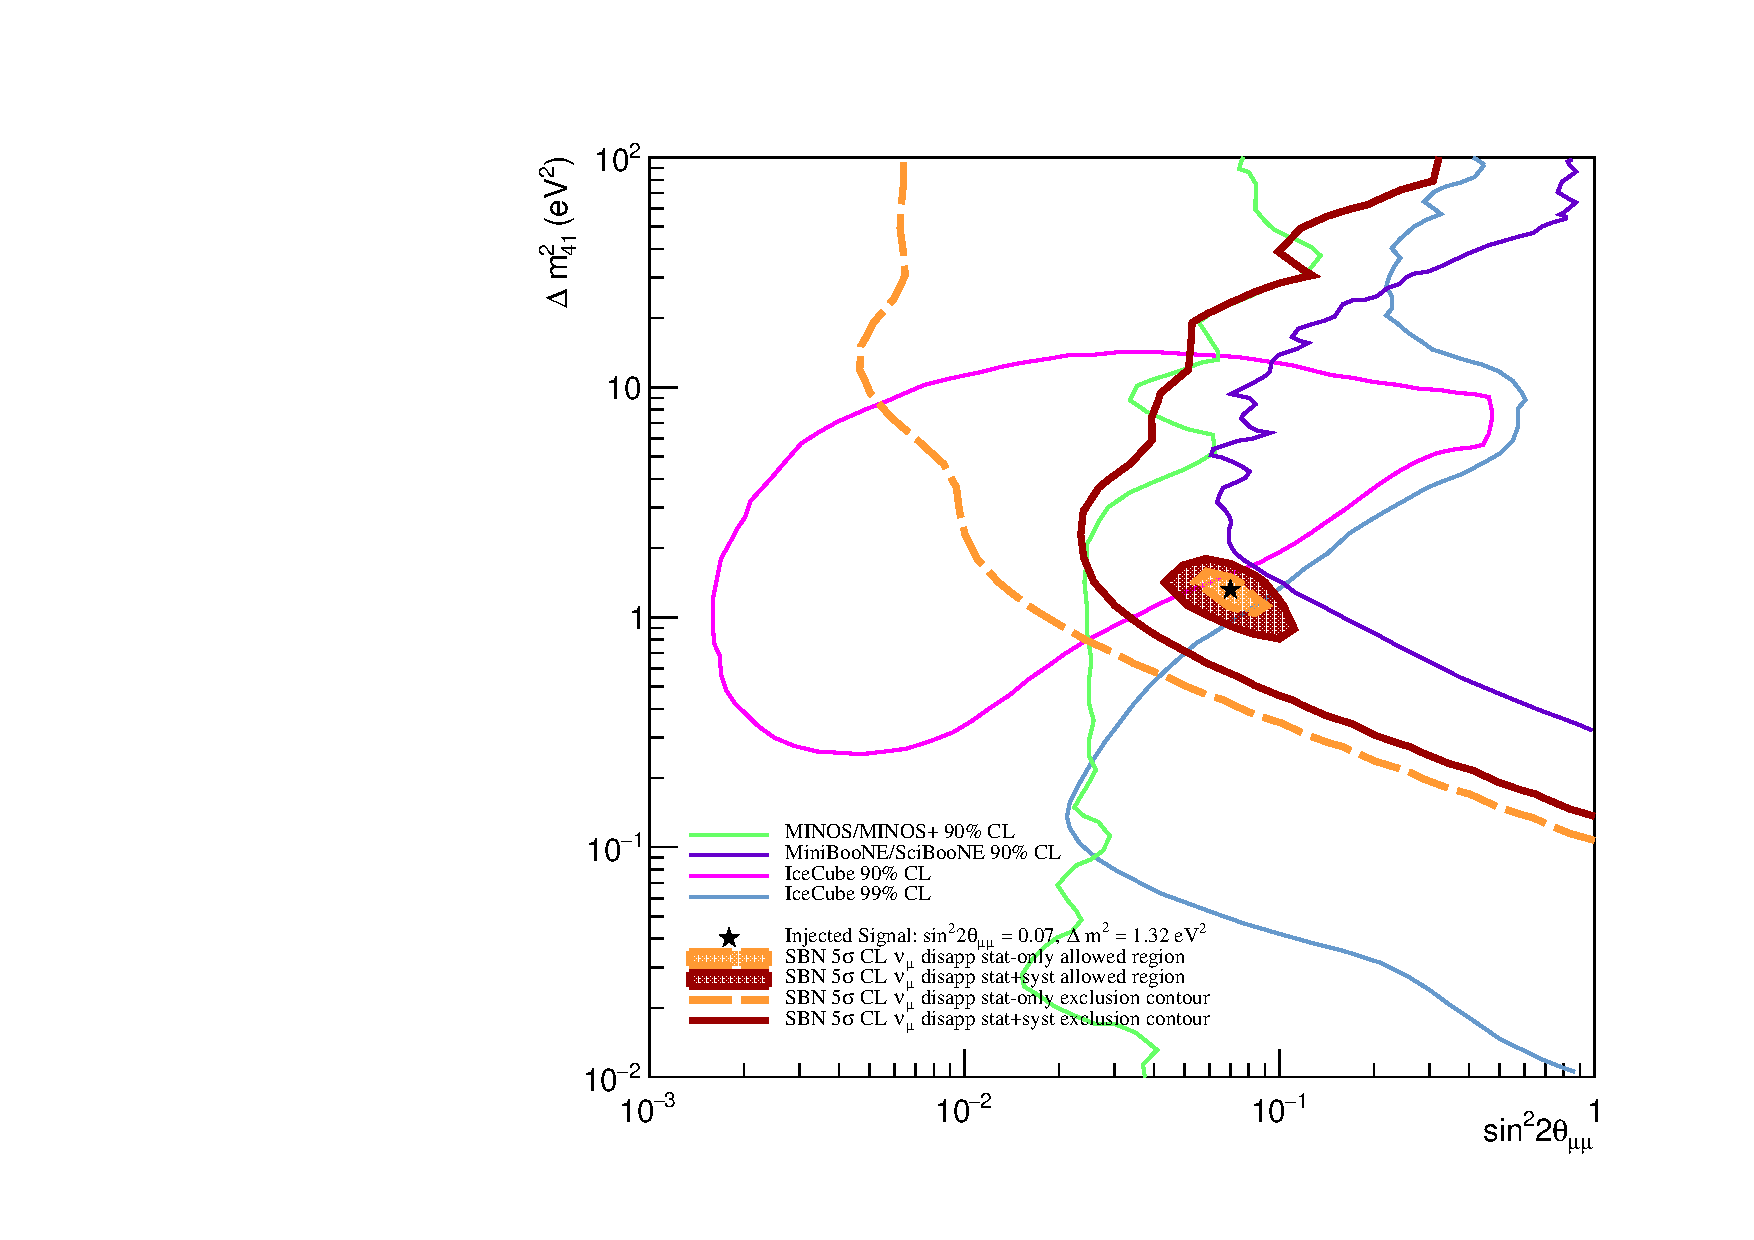
\includegraphics[width = \largefigwidth]{figures-chap6/overlays/valor_overlays_numu_disapp.pdf}
    \caption[\numu disappearance contours with external limits.]{\numu disappearance exclusion contours and allowed regions for the stat only case and with flux and interaction systematic uncertainties included. External limits from the MiniBooNE/SciBooNE, MINOS/MINOS+ and IceCube experiments have been overlayed \cite{MiniBooNE/SciBooNE_numu_disapp_contour}\cite{MINOS_numu_disapp_contour}\cite{IceCube_numu_disapp_contour}. (The confidence intervals for each contour are shown in the legend and it should be noted that those from external limits are not the same as those from the contours produced for the \gls{sbn} program.)}
    \label{fig:numu_disapp_global_sensitivity}
\end{figure}

\newpage
\section*{\texorpdfstring{Impact of Efficiency Systematics on \numu Disappearance Sensitivities}{Impact of Efficiency Systematics on numu Disappearance Sensitivities}}


The impact of fully correlated uncertainties up to 10\% are shown on the left of \FigureRef{fig:numu_corr_uncorr_error} whilst keeping the uncorrelated uncertainty at 0\%. The right plot shows the impact of increasing the uncorrelated uncertainties uniformly across all bins with a fixed correlated uncertainty of 2\%. It follows that for even relatively large correlated uncertainties the impact on the sensitivity is minor and that any reduction in sensitivities will be largely dominated by the uncorrelated uncertainty. 

\begin{figure}[!h]
    \centering
    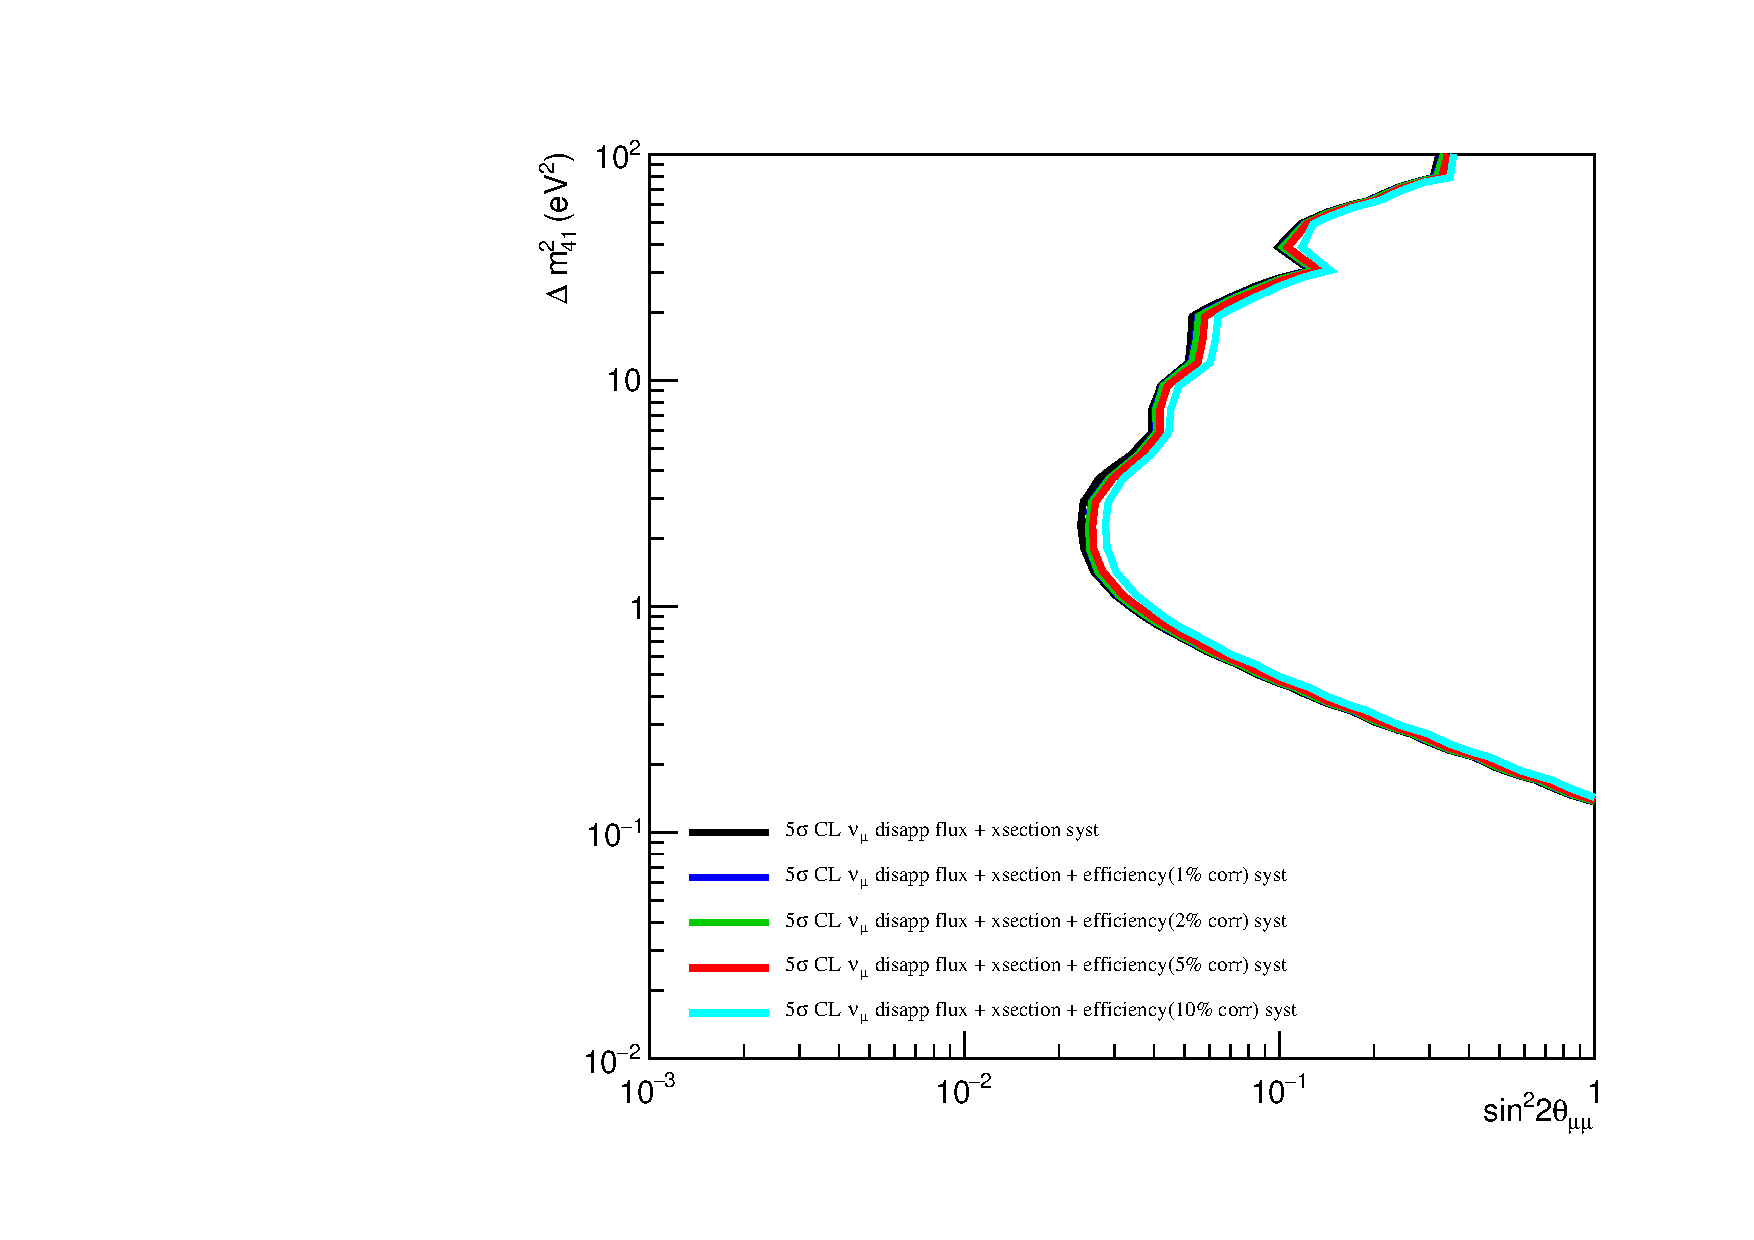
\includegraphics[width = 0.49\textwidth]{figures-chap6/exclusion_contours/efficiency_systematics/numu_disapp_Xpct_cor.pdf}
    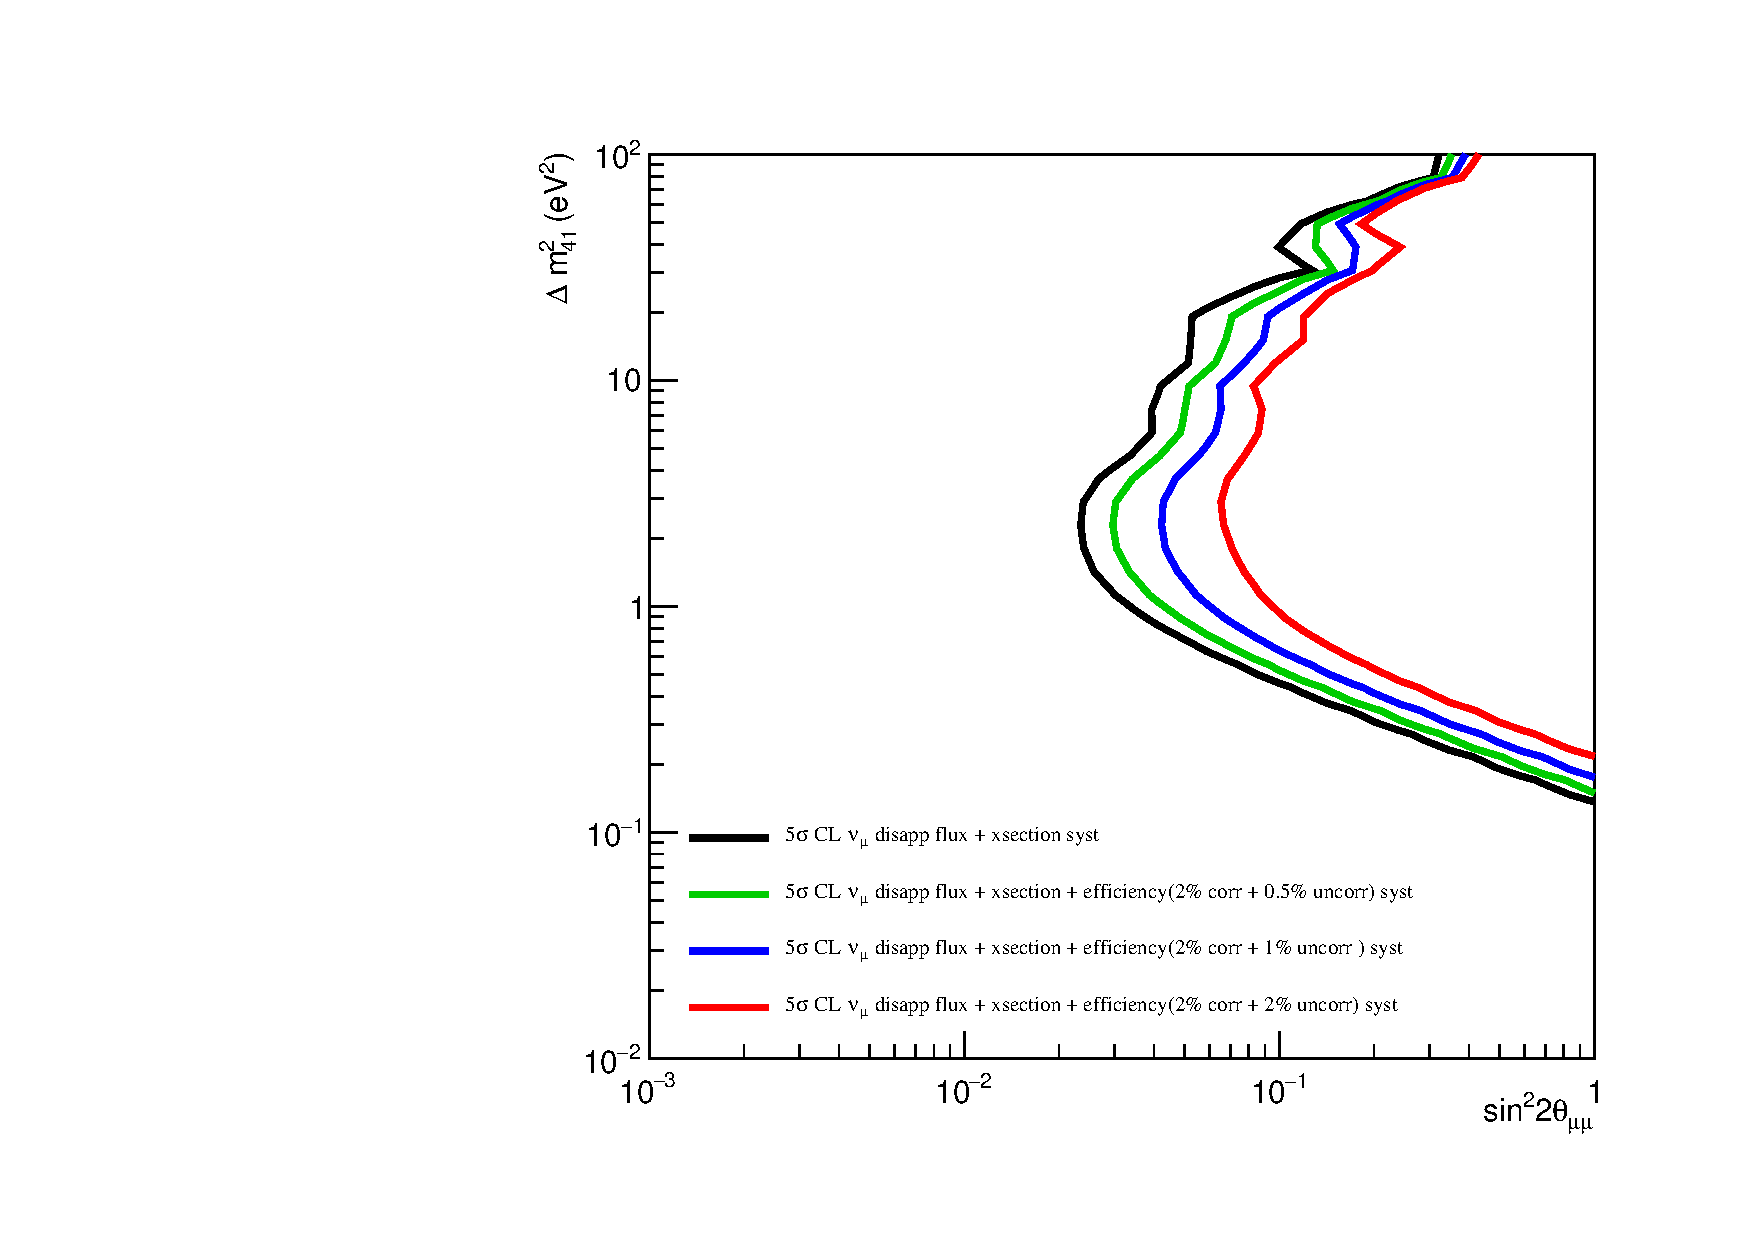
\includegraphics[width = 0.49\textwidth]{figures-chap6/exclusion_contours/efficiency_systematics/numu_disapp_2pct_cor_Xpct_uncor.pdf}
    \caption[Impact of correlated and uncorrelated efficiency systematics on the \numu disappearance channel.]{The impact on the \numu disappearance exclusion sensitivity by applying fully correlated uncertainties ranging from 1\% to 10\% to all bins (Left) and by applying a fixed 2\% fully correlated uncertainty with additional uncorrelated uncertainty ranging from 0.5\% to 2\% across all bins (Right). }
    \label{fig:numu_corr_uncorr_error}
\end{figure}

\FigureRef{fig:numu_uncorr_det} shows the impact of applying a 2\% uncorrelated uncertainty only to each of the \gls{sbn} detectors one at a time. The \gls{microboone} detector has a minor impact at around $\Delta m ^2_{41} = 10$ eV$^2$ and close to no impact at small and large $\Delta m ^2_{41}$ values. The \gls{icarus} detector has a larger impact for most $\Delta m ^2_{41}$ values but again only has a minor contribution at very large $\Delta m ^2_{41}$ values. Across most $\Delta m ^2_{41}$ values greater than $\sim$0.5 eV$^2$, \gls{sbnd} dominates the sensitivity. At values below 0.5 eV$^2$, the reduction in sensitivity due to \gls{sbnd} and \gls{icarus} are comparable. This point is emphasised in \FigureRef{fig:numu_uncorr} where the fully correlated uncertainty is fixed at 2\% and the uncorrelated uncertainty is set to 2\% for one of the three \gls{sbn} detectors whilst being set to 0.5\% for the other two detectors. The contour where \glspl{sbnd} uncorrelated uncertainty is set to 2\% looks similar to the corresponding contour in \FigureRef{fig:numu_uncorr_det}. It has been shown that the uncorrelated component of the uncertainty has a large impact when compared to the correlated component and that any efficiency uncertainties impact \gls{sbnd} more than the other two detectors so this result ought to be expected. Similarly, the two contours where uncorrelated uncertainty is set to 2\% for \gls{microboone} and \gls{icarus} are pulled towards the \gls{sbnd} contour since despite it having a smaller associated uncorrelated uncertainty, it will still contribute significantly. 

\begin{figure}[!h]
    \centering
    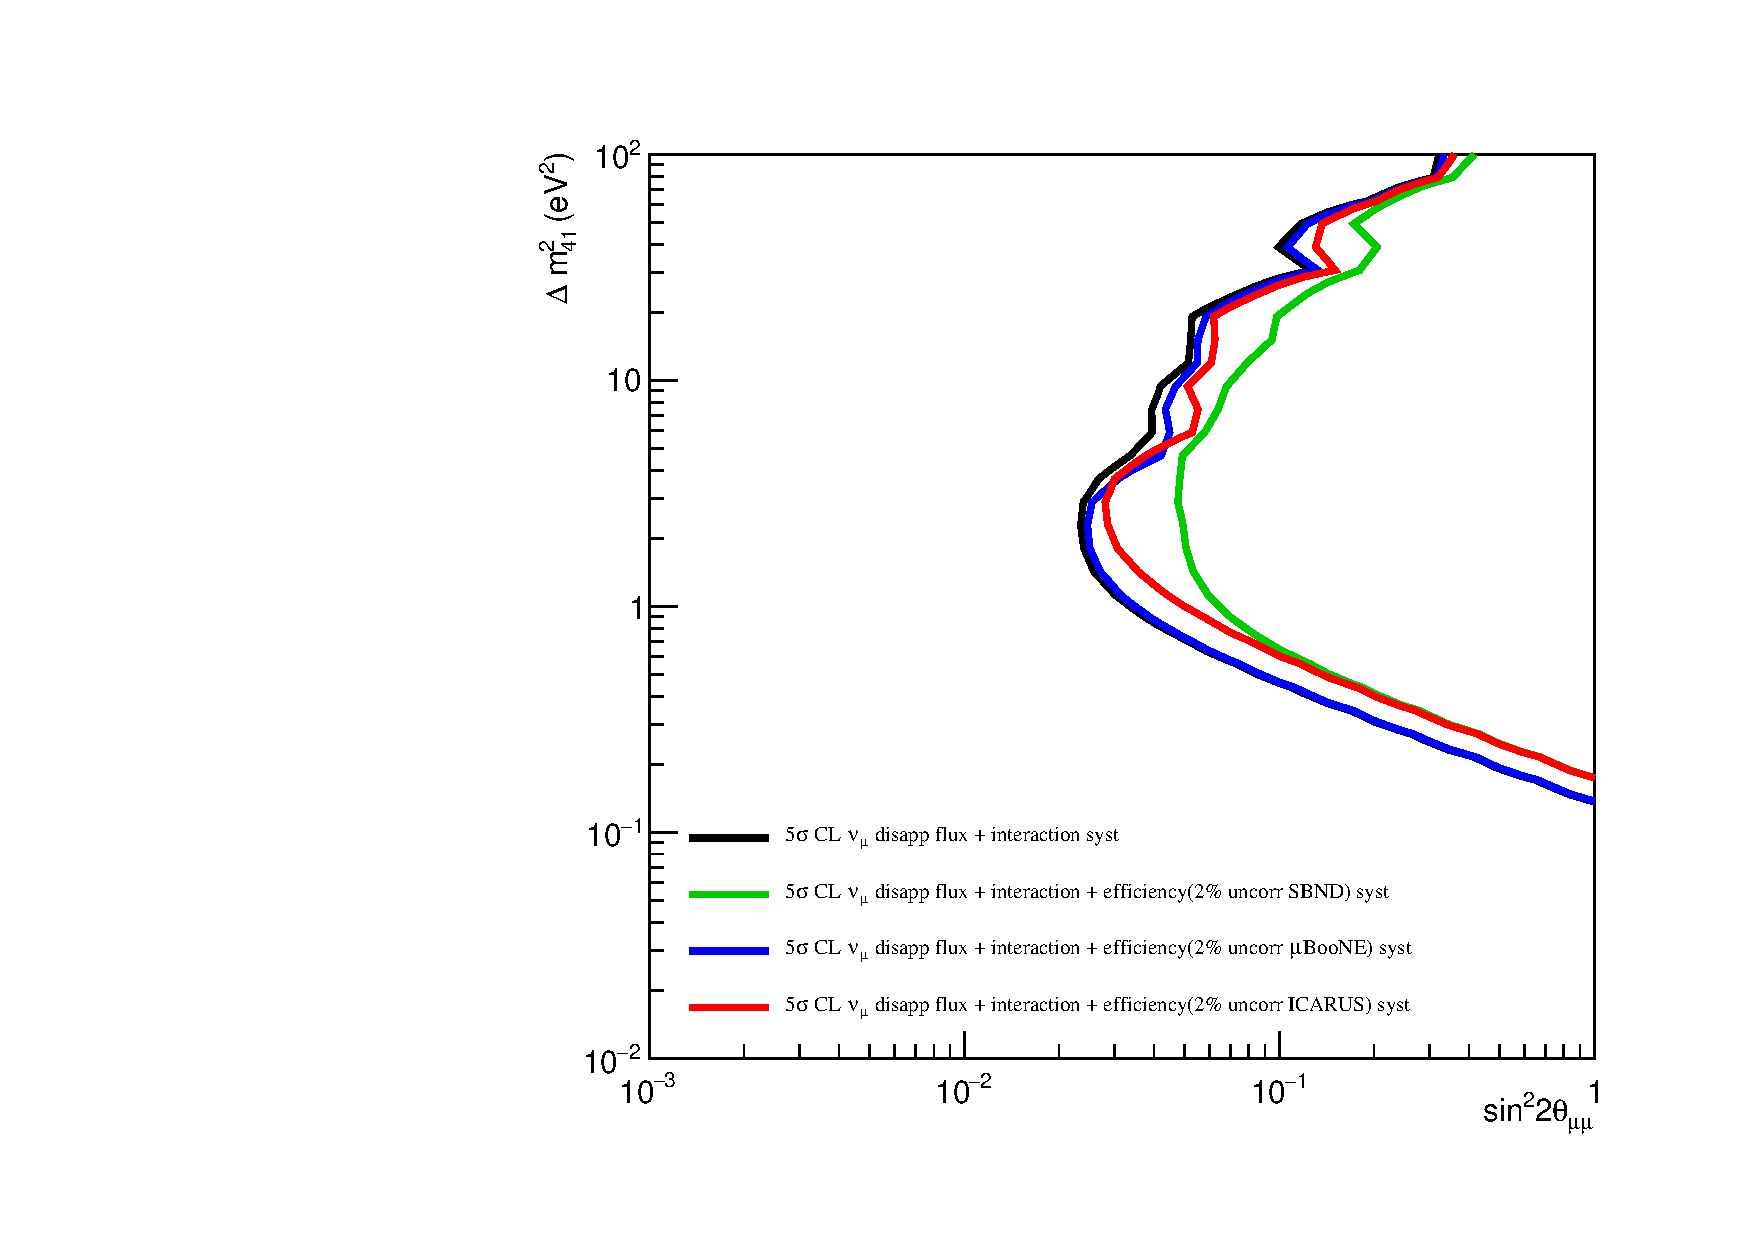
\includegraphics[width = \largefigwidth]{figures-chap6/exclusion_contours/efficiency_systematics/numu_disapp_2pct_uncor_per_detector.pdf}
    \caption[Impact of a 2\% uncorrelated efficiency systematic on the \numu disappearance channel for each individual detector.]{The impact on the \numu disappearance exclusion sensitivity by applying a 2\% uncorrelated efficiency uncertainty to a single one of the three \gls{sbn} detectors.}
    \label{fig:numu_uncorr_det}
\end{figure}

\begin{figure}[!h]
    \centering
    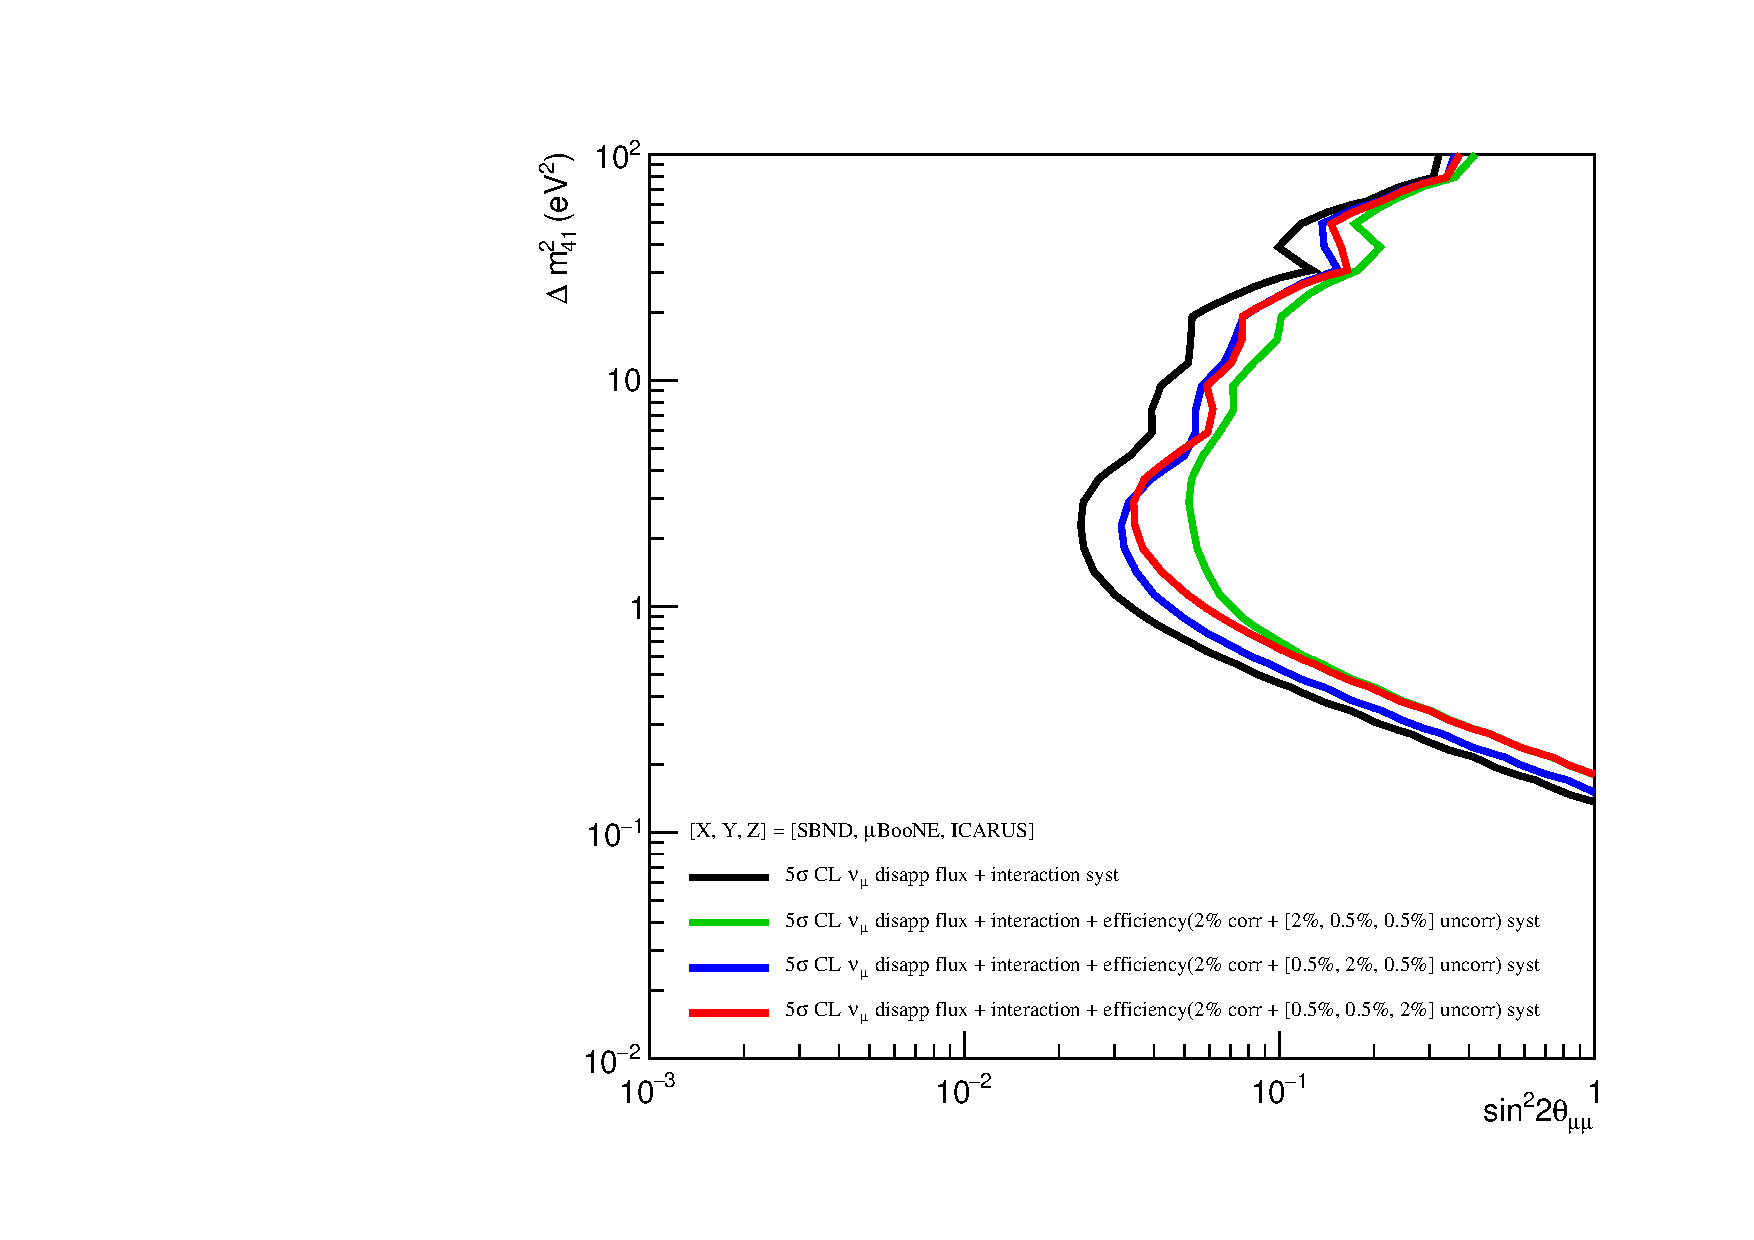
\includegraphics[width = \largefigwidth]{figures-chap6/exclusion_contours/efficiency_systematics/numu_disapp_2pct_cor_2pct_X_05pct_other_per_detector_uncor.pdf}
    \caption[Impact of a 2\% uncorrelated efficiency systematic for one detector and 0.5\% for the other two on the \numu disappearance channel.]{The impact on the \numu disappearance exclusion sensitivity by applying a 2\% fully correlated efficiency uncertainty for each of the \gls{sbn} detectors and a 2\% uncorrelated uncertainty for one of the detectors and a 0.5\% uncorrelated uncertainty for the other two detectors. This is repeated for each of the detectors. The associated covariance matrix used for the case where \glspl{sbnd} uncorrelated uncertainty was set to 2\% is shown in the bottom left plot of \FigureRef{fig:efficiency_cov_matrices}.}
    \label{fig:numu_uncorr}
\end{figure}

\newpage
%Instead of exploring the impact from fully uncorrelated uncertainties or a constant uncorrelated uncertainty across all bins in a detector,
\FigureRef{fig:numu_bulk_uncorr} considers the case where a single set of bins are poorly constrained using the same scheme outlined in \SectionRef{sec:Impact of Additional Efficiency Systematics}. In each case, the uncorrelated uncertainty for the bins of interest are again set to 2\% in each of the \gls{sbn} detectors, whilst the rest of the uncorrelated uncertainties are set to 0.5\% and the fully correlated uncertainty is fixed at 2\%. Increasing the uncertainty associated with the background bins has the smallest impact whereas increasing the uncertainty for the high and low energy bins has the largest impact at large and small $\Delta m^2_{41}$ respectively. The peak energy bins also contribute significantly around $\Delta m^2_{41}$ equal to 1 eV$^2$ and 10 eV$^2$. 


\begin{figure}[!h]
    \centering
    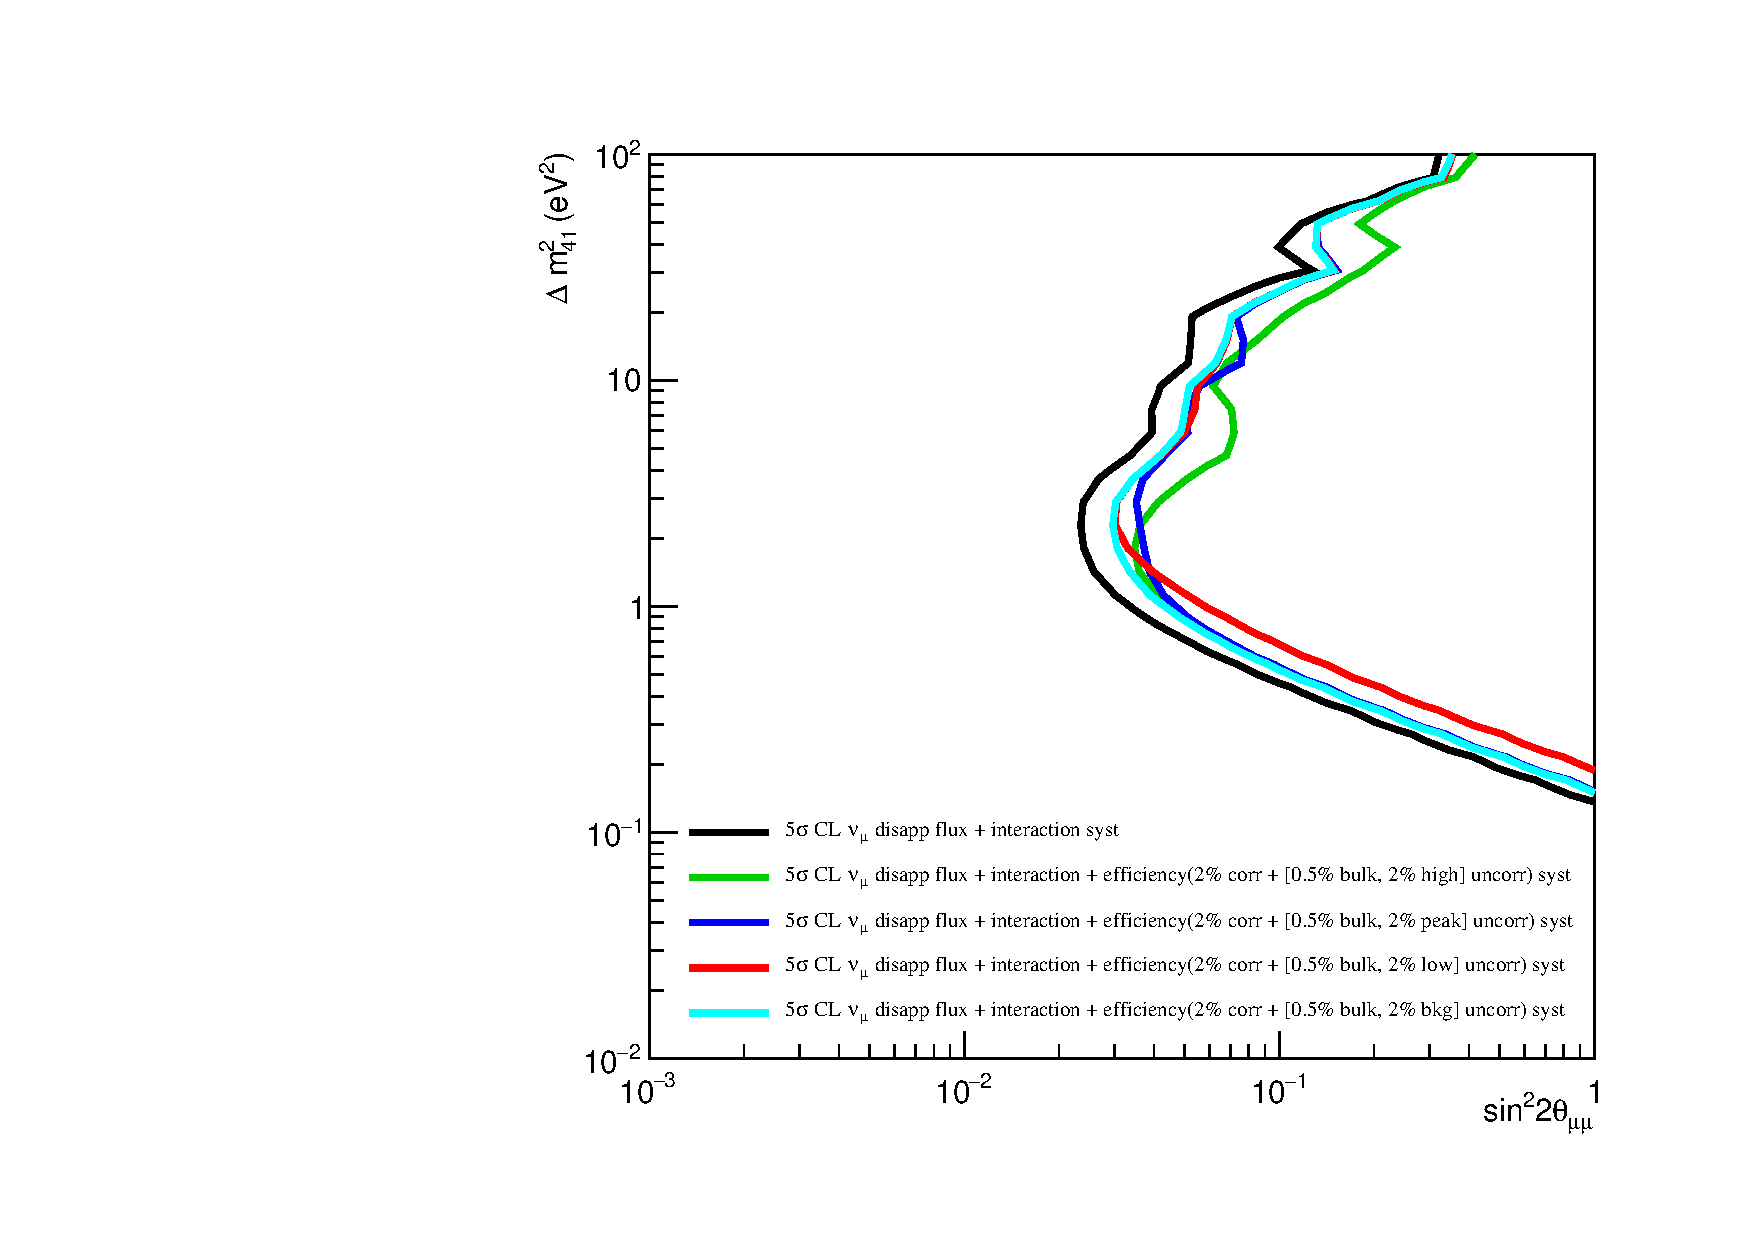
\includegraphics[width = \largefigwidth]{figures-chap6/exclusion_contours/efficiency_systematics/numu_disapp_2pct_cor_05pct_bulk_2pct_X_uncor.pdf}
    \caption[\numu disappearance with poorly constrained efficiency systematic for a set of bins.]{The impact on the \numu disappearance exclusion sensitivity by applying a 2\% fully correlated efficiency uncertainty for each of the \gls{sbn} detectors and a 0.5\% uncorrelated uncertainty for all but a single set of bins where the uncorrelated uncertainty is set to 2\%. The 'peak' energy bins are defined as those covering an energy range of [0.6,~1.0] GeV. The 'high' and 'low' energy bins are defined as those covering energies above and below the peak energy respectively and the 'bkg' bins are all the bins associated with background events. The set of bins of interest are applied to each of the three detectors and the covariance matrix for where the peak energy bins are the ones in question is shown in the bottom right plot of \FigureRef{fig:efficiency_cov_matrices}.}
    \label{fig:numu_bulk_uncorr}
\end{figure}







%% Big appendixes should be split off into separate files, just like chapters
%\input{app-myreallybigappendix}
